% !TEX root = paper.tex

\section{InferSpark System}
\label{sec:optimization}

\begin{figure*}[th]
\centering
    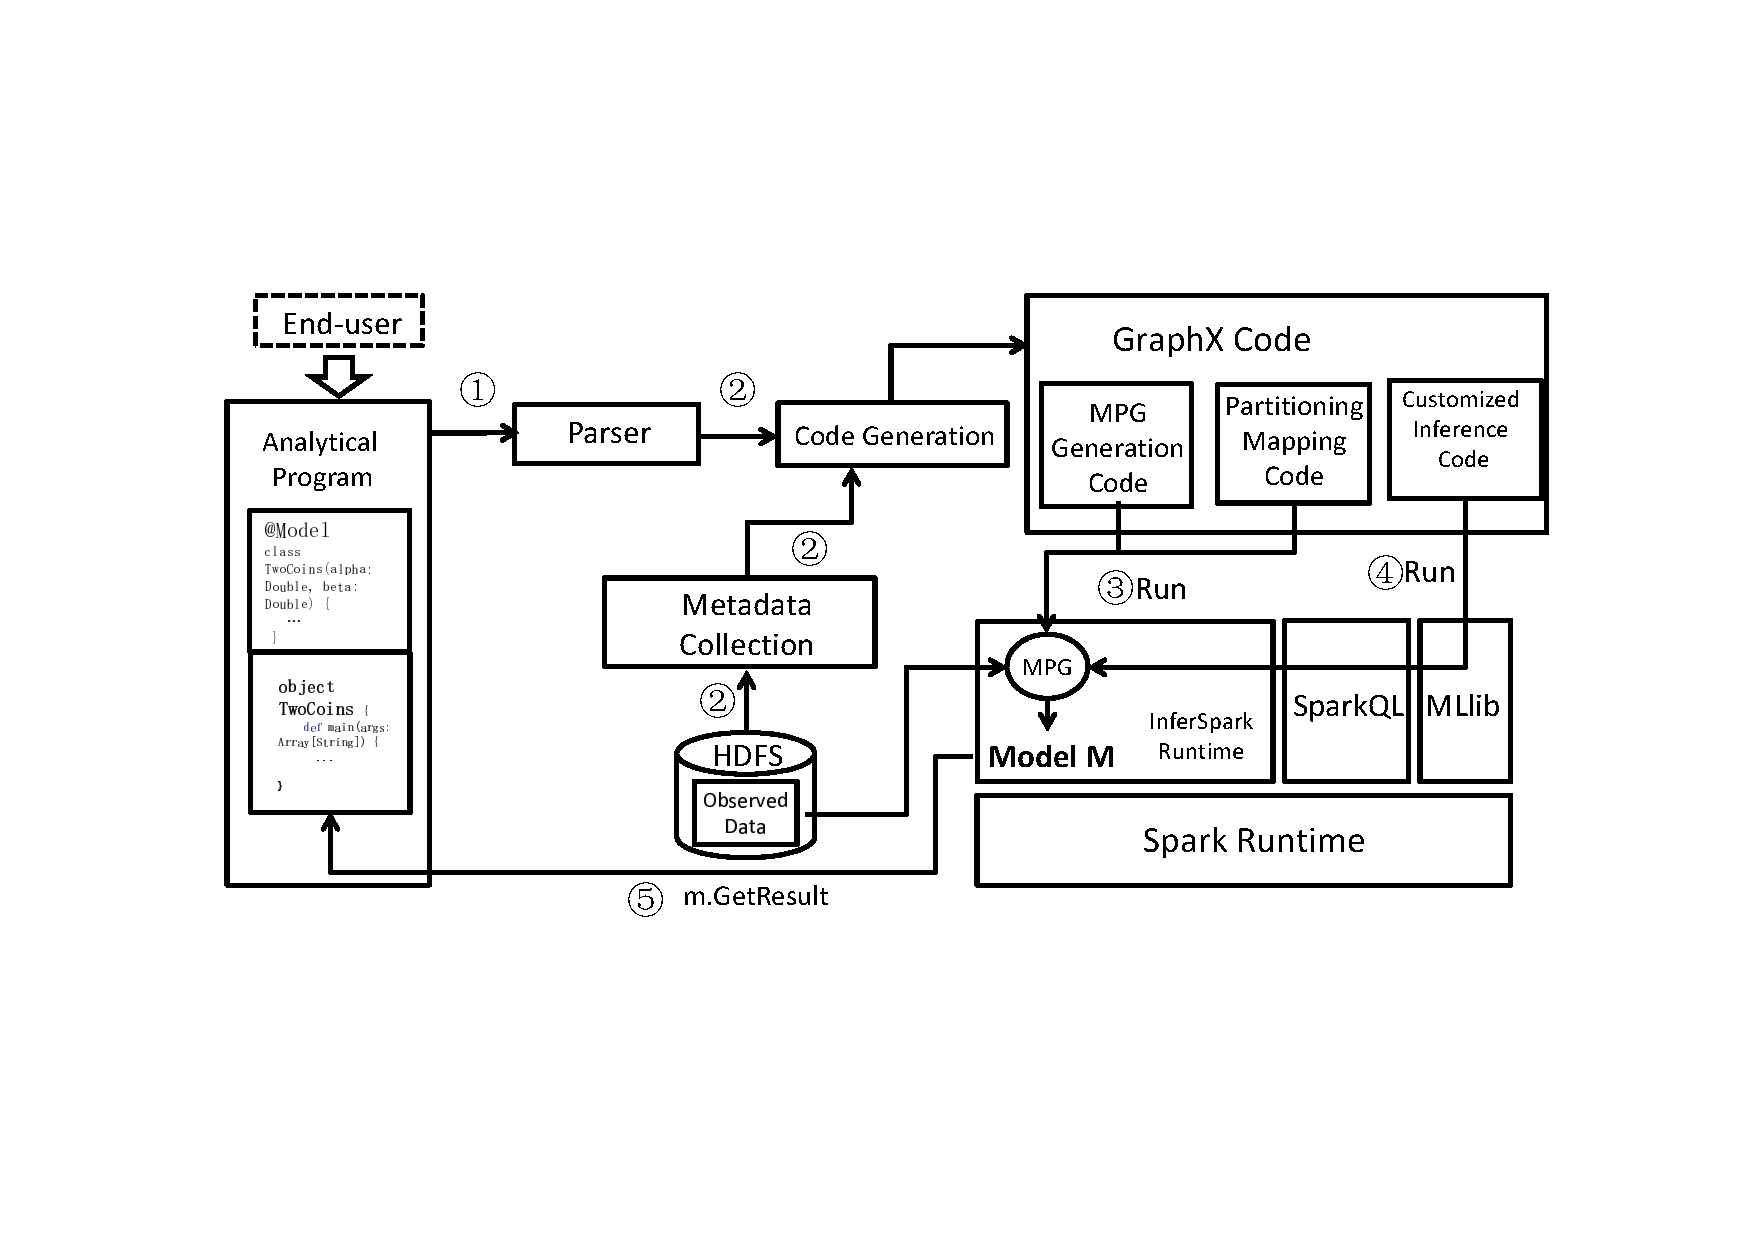
\includegraphics[width=1.4\columnwidth]{figs/InferFra1}
    \caption{InferSpark Architecture}
    \label{fig:workflow}
\end{figure*}


\figref{fig:workflow} shows the architecture of the InferSpark system.
When encountering an InferSpark program within a Spark program,
the Spark runtime will hand over the control the InferSpark system.
The InferSpark system will
\protect \circled{1}
first parse the InferSpark program,
then it will \protect \circled{2} carry out \emph{code generation}
to generate three pieces of code:
(a) code that generates the message passing graph (MPG) based on the model in PGM and the characteristics of the observed data (e.g., the number of records in the data),
(b) code that encodes the best partitioning mapping for the MPG that will be generated by (a),
and (c) code that embed an inference algorithm with all details.
More specifically,
InferSpark adopts two popular inference algorithms,
VMP \cite{vmp} and Gibbs sampling \cite{gibbs},
which are both
implementable through message passing.
VMP, for example,  expands a PGM into a message passing graph (MPG)
and then carries out the inference
 by passing messages between nodes in the MPG
  and updating posterior beliefs using local operations at each node.
Therefore,
Code (a) is for MPG construction
and Code (c) is a concrete inference algorithm
with all messages (which are a set of expected values between \EL{ help++++++} defined.


In order to increase portability,
the code generation module generates code based on GraphX API.
Nevertheless,
the InferSpark system executes the generated code
using its own InferSpark runtime
(\circled{3} and \circled{4})
instead of the GraphX runtime
because the GraphX runtime is general
but we observe that the graphs, more specifically, the message passing graphs,
are highly structured, where a specialized runtime engine designated for that kind of graphs can obtain substantial performance boost
and can thus speed up the entire inference process.

Within the InferSpark runtime,
an in-memory MPG would first be generated
and physically partitioned
\circled{3}
and then the inference algorithm
would  \circled{4} infer the unknowns
 by
passing messages among nodes of the MPG
sifting through the observed data in the HDFS.


When the inference process is done, the InferSpark system
would \circled{5}
return the control back to the Spark runtime  to execute the subsequent code
and serve any queries about the resulting model from Spark runtime on demand.










%\KZ{Give an overview of the archi \figref{fig:workflow} here.}
%\JL{First the user would define a custom model by using our inferSpark programming language, then our parser would parse the input code and generated the corresponding code for the model. Meanwhile, the user should give some parameters such as the template number of the model or the observed data when writing the program, therefore provide the metadata which would be used in the next step. Next, we would combine the template model with the given metadata and then do code generation for the algorithm. We have a runtime scala file which would read the model and meta data from input and then generate different codes for different models automatically. In addition to this, we also optimized the GraphX API in Spark so that we could run algorithm at a higher speed. Then we would run this generated program on the top of Spark platform, after which the user would get a result such as the posterior of some random variables. }
%\subsection{Model Construction and Metadata Collection}

\subsection{Parsing}
An input InferSpark program is first parsed and separated into two parts:
the model definition (``{\sf @Model} class TwoCoins'' in
\figref{fig:two_coins_modeldef}) and
the ordinary scala program (``{\sf object Main}'' in
\figref{fig:two_coins_modeldef}). The model definition is analyzed and
transformed into valid scala classes that define a Bayesian
network constructed from the model definition
(e.g., \figref{fig:two_coins_bn1}) and the inference/query API.
Note the Bayesian network
constructed at this stage is only a template.


\subsection{Code Generation}


\subsubsection{MPG Construction Code Generation}
\begin{figure}[h]
\centering
\includegraphics[scale=0.4]{figs/two_coins_bn1.eps}
\caption{Bayesian Network Template Constructed from the Two-coin Model}
\label{fig:two_coins_bn1}
\end{figure}
%The model construction module separates the model part
%out, and transforms it into a Bayesian network template.
%%The algorithm matching module selects the applicable inference algorithm
%%(e.g. variational message passing).
%The template is
%then instantiated with parameters and metadata from the input data at runtime
%by the code generation module, which produces the inference code. These are
%then executed on the Spark distributed engine to produce the final posterior
%distributions.
%
%
%\KZ{Say a bit about metadata collection module?}
%\JL{Metadata such as the observed variables and the plate sizes missing from the
%Bayesian networks are collected at run time. In the two-coin
%model, an instance of the model is created via the constructor invocation (e.g.
%``{\sf val m = new TwoCoin(1.0, 1.0)}'' on line 10 of \figref{fig:two_coins_modeldef}). The constructor call provides
%the missing constants in the prior distributions of $\pi$ and $\phi$.
%For each random variable defined in the model definition,
%there is an interface field with the
%same name in the constructed object. Observed values are provided to InferSpark
%by calling the ``{\sf observe}'' (line 11 of \figref{fig:two_coins_modeldef})
%API on the field.
%There, the user provides an RDD of observed outcomes ``{\sf xdata}'' to InferSpark by calling
%``{\sf m.x.observe(xdata)}''. The  {\sf observe} API also triggers
%the calculation of unknown plate sizes.
%In this case, the size of plate surrounding $z$ and $x$ is
%automatically calculated by counting the number of elements in the RDD.}
In this step, the code generator of the InferSpark system
aims to produce code that would generate a message passing graph from the Bayesian network
given by the parser.
%convert the Bayesian network to a message passing graph on GraphX,
%InferSpark needs to construct a VertexRDD and an EdgeRDD. This step generates
%the MPG construction code specific to the data.
\figref{fig:two_coins_mpg_constr_code} shows the MPG construction code
generated for the two-coin model.
The vertices are constructed by the union
of three RDD's, one of which from the data and the others from
parallelized collections (lines 8 and line 9 in \figref{fig:two_coins_mpg_constr_code}).
The edges are built from the data only.
A partition strategy specific to the
data is also generated in this step.




%\begin{figure}[h]
%%class TwoCoinsPS extends PartitionStrategy {
%%	override def getPartition /**/
%%}
%\begin{lstlisting}
%def constrMPG() = {
%	val v1 = Categorical$13$observedValue.mapPartitions{
%		initialize z, x */
%	}
%	val v2 = sc.parallelize(0 until 2).map{ /* initialize phi */ }
%	val v3 = sc.parallelize(0 until 1).map{ /* initialize pi */ }
%	val e1 = Categorical$13$observedValue.mapParititons{
%		/* initialize edges */
%	}
%	Graph(v1 ++ v2 ++ v3, e1).partitionBy(new TwoCoinsPS())
%}
%\end{lstlisting}
%\caption{Generated MPG Construction Code}
%\label{fig:two_coins_mpg_constr_code}
%\end{figure}

\begin{figure}[h]
%class TwoCoinsPS extends PartitionStrategy {
%	override def getPartition /**/
%}
\begin{lstlisting}
def constrMPG() = {
	val v1 = observed_data.metadata.mapPartitions{
		initialize vertex z, x by the metadata of observed data */
	}
	val v2 = sc.parallelize(0 until phi).map{ /* initialize vertex phi */ }
	val v3 = sc.parallelize(0 until pi).map{ /* initialize vertex pi */ }
	val e1 = observed_data.metadata.mapParititons{
		/* initialize edges */
	}
	Graph(v1 ++ v2 ++ v3, e1)
}
\end{lstlisting}
\caption{Generated MPG Construction Code}
\label{fig:two_coins_mpg_constr_code}
\end{figure}


%Constructing the
%message passing graph of the Bayesian network is not trivial because different
%types of random variables have different initialization methods and different
%data sources. The initialization of the outcomes $x$ in the two-coin model is
%fixing its distribution to a point categorical distribution at the observed
%outcome and randomly initialize the incoming messages while the initialization
%of the choice of coins $z$ is to randomly initialize the parameters of its
%approximate marginal posterior distribution. The data source of $x$ is the
%observed outcomes while $z$ does not have data source. The initialization of
%EdgeRDD is also nontrivial because the links between different random
%variables have different structures. Inferspark finds a transformation plan
%for the MPG construction. A possible plan for the two-coin model is shown in
%\figref{fig:two_coins_mpg_construction_plan}.
%
%\begin{figure}[h]
%	\centering
%	\includegraphics[width=0.45\textwidth]{figs/two_coins_mpg_construction_plan.eps}
%	\caption{MPG Construction Plan of Two-Coin Model}
%		\label{fig:two_coins_mpg_construction_plan}
%\end{figure}

%In a typical GraphX application, the property graph has homogeneous vertex
%properties and edge properties. In the shortest distance application, the
%vertex properties are shortest distance from the origin and edges properties
%are weights. The EM algorithm implementation for LDA in Mllib, which only
%computes the Maximum A Posterior rather than the full posterior, uses the
%vertex properties as topic counts and edge propertices as word counts. However,
%the message passing graph of the VMP algorithm generally have heterogeneous
%vertex properties and edge properties. In the LDA case, we have three types of
%vertecies: observed categorical mixture, unobserved categorical variable and
%unobserved dirichlet variable. The observed categorical mixture needs to store
%the messages from parents and the observed value while the other two types need
%to store the sufficient statistics. The edges also have differnt structures.
%There's one-to-one correspondence between $z$ and $w$ while $w$ are fully
%connected to $\phi$. Therefore, the compiler need to create an unrolling plan
%so that the graph is correctly initialized. In the LDA case, a possible plan is
%to first map from the observations of x to create vertecies for $\theta$, $z$
%and $x$ and use a parallelized range to create verticies for $\phi$. Another
%possibility is to separately initialize each set of variables.  We try to
%minimize the overhead of union by merging the initialization of variables as
%much as possible.


%\begin{figure}[h]
%\centering
%\begin{lstlisting}
%class TwoCoins(alpha: Double, beta: Double) extends ModelBase {
%	val synval$internal$parent: Array[Int] = /**/
%	var Categorical$13$isObserved: Boolean = _
%	class Categorical$13$Inferface extends RandomVariable {
%		def observe(obs: RDD[Long]) = /* ... */
%		def getResult(): RDD[CategoricalResult] = /* ... */
%	}
%	val x = new Categorical$13$Interface()
%	/* ... */
%}
%\end{lstlisting}
%\caption{Bayesian Network Code}
%\label{fig:two_coins_stage1code}
%\end{figure}
%
%The Bayesian network source code is then compiled with the
%ordinary scala program into bytecode. This bytecode will generate the
%inference code of the VMP algorithm for the model on GraphX in
%the next 4 steps.
%
%The InferSpark model definition is a scala definition with ``@Model''
%annotation. The scala parser first separates the model definition from other
%part of the program (i.e. user program). A Bayesian network is then constructed
%according to dependencies between the random variables in the model definition.
%\figref{fig:lda_bn1} is the Bayesian network constructed from the LDA model
%definition. Some information only available at runtime are missing from the
%Bayesian network, e.g. the number of topics $K$, the observed words $w$, etc.
%At this step, the analyzer also verifies that the model is in the
%exponentail-conjugate family and rejects unsupported model definitions. After
%the construction, the Bayesian network is stored in the compiled program for
%later steps to process.

%\begin{figure}[!h]
%	\centering
%	\includegraphics[scale=0.3]{figs/lda_bn1.eps}
%	\caption{Bayesian Network Constructed From the Model Definition}
%	\label{fig:lda_bn1}
%\end{figure}

%When the user provide the observed random variables such as the words in the
%LDA model, the number of documents and the number of words in each document
%can be inferred from the data. This is different from most libraries in that
%they require the user to explicitly set the numbers or to transform the data
%into a library-specific format. InferSpark also tries to verify that the user
%have provided consistent data. For example, InferSpark will report an error,
%if the user provides data to both the topics $z$ and the words $w$ but they
%have differnt sizes.

In this step, the code generator of the InferSpark system
aims to produce code for carrying out the inference.
For the sake of discussion,
we assume the VMP algorithm is in use.

This step annotates the messages and vertex updates of the algorithm to the
Bayesian network from previous step and we call the resuling graph as message
passing graph.

The VMP algorithm is expressed as sending messages of functions of sufficient
statistics of random variables and updating the sufficient statistics by
aggregating the messages. The messages are sent in both direction of the edges
in the Bayesian network. The vertices are updated by aggregating incoming
messages. For the Dirichlet random variables, the update is simply adding
together all the messages. The unobserved Categorical random variable $z$ is
updated by normalizing the sum of the messages. The observed Categorical
mixtures $w$ have nothing to update but have to compute the new messages to $z$
and $\phi$ according to the incoming messages.

\begin{figure}[h]
	\centering	
	\includegraphics[scale=0.3]{figs/lda_mpg.eps}
	\caption{Message Passing Graph of LDA}
	\label{fig:lda_mpg}
\end{figure}


The messages in the VMP algorithm are sent in both directions. The messages
along the edge only depend on the sender but the messages in the reverse
direction may also depend on other parents' message.  For example, the message
along the edge from $z$ to $w$ only depends on the sufficient statistics of
the Categorical variable $z$, but the reverse one will depend on the
topic-word distributions' messages. The original VMP algorithm assumes that
only one vertex may be updated in each step and the messages that the vertex
depends on are always up-to-date.  However, this poses two challenges when
implementing it as a distributed message passing algorithm. First, we have to
relax the assumption of one vertex in each step to increase parallelism
without violating the correctness of the algorithm. In the LDA example,
Updating all the random variables at the same time does not guarantee to
optimize the ELBO but we can update all the topics at the same time because it
is equivalent to sequentially update each of the topics. Secondly, vertecies
that have not been updated could send messages that depends on stale messages.
If updates to the topics $z$ are immediately followed by updates to the
topic-word distributions $\phi$, the messages from $w$ to $\phi$ will depend
on the messages sent from $z$ to $w$ prior to the update of $z$ instead of the
new messages from $z$ to $w$. Therefore, we choose an update schedule that is
equivalent to sequential updates to ensure the correctness of the algorithm.


\subsubsection{Inference Code Generation}

\begin{figure}
\centering
	\includegraphics[width=0.35\textwidth]{figs/two_coins_msg.eps}
	\caption{Bayesian Network with Messages for Two-coin Model}
	\label{fig:two_coins_msg}
\end{figure}

%When the user calls ``{\sf infer}'' API (line 12 of
%\figref{fig:two_coins_modeldef}) on the model instance, InferSpark checks
%whether all the missing metadata are collected.
%
%If so, it proceeds to
%the code generation module.
%\KZ{Introduce three diff algos: VMP, Gibbs and EP. We might need to discuss
%the basic parallel version of these algos separately here.}
%\JL{ We have two algorithms: VMP and Gibbs Samplimg. We would introduce them briefly. They would do approximate inference on the Bayesian network with messages we derived manually, resulting in \figref{fig:two_coins_msg}. The expressions that
%calculate the messages (e.g., $E_{Q_\pi}[\ln \pi]$) depend on not only the
%structure of the Bayesian network and whether the vertices are observed or
%not, but also practical consideration of efficiency and constraints on GraphX and Spark.
%}


%\subsection{MPG Construction Code Generation}

In addition to generating code to build the large message passing graph,
the codegen module also generates code for VMP iterative inference.
InferSpark, which
distributes the computation, needs to create a schedule of parallel updates
that is equivalent to the original VMP algorithm, which only updates one vertex
in each iteration.  Different instances of the same random variables can be
updated at the same time. An example update schedule for the two-coins model is
($\pi$ and $\phi$) $\rightarrow$ $x$ $\rightarrow$ $z$ $\rightarrow$ $x$. VMP inference code that enforces the update
schedule is then generated. % \ERIC{how to derive this indeed?}

InferSpark currently include the VMP algorithm while other inference algorithms
such as Belief Propagation, Gibbs Sampling and etc. will be added to it in
order to support inference on a wider range of Bayesian networks. We will also
publish a high-level language for implementing inference algorithms and
specifying what models the algorithms apply to.  Algorithm developers are
welcomed to add new algorithms whenever existing ones do not fit the needs of
end-users. Algorithm matching module searches for an applicable algorithm among
both the built-in and the developer-suppied inference algorithms while the new
CodeGen module transforms the algorithm into a Spark program and handles all
the low-level optimizations. These two modules are similar to efforts like
SystemML, MLI, which targets algorithm developers, but an integrated part of
InferSpark.

%With all the information collected and calculated in previous steps,
%implementation of the inference algorithm as a GraphX program is generated,
%compiled and then executed. User can retrieve the posterior distributions as
%VertexRDDs through API calls.
\subsubsection{Partitioning Code Generation}
The performance of the inference algorithm highly
depends on how we partition the message passing graphs.
Vertex-cut partitioning has the advantage
of having the communication and storage overhead directly proportional to the sum of the number of machines spanned by each vertex \cite{graphX}.
Therefore, if we are able to find a partitioning strategy that evenly assigning edges to machines
and minimizing the number of machines spanned by each vertex,
the inference time could be significantly reduced.

When the discussion reaches this point,
readers might have discovered that
message passing graphs, unlike many real-world graphs,
are highly \emph{structured}.
That is reasonable because a message passing graph
is always expanded from a PGM.
In the following, we first analyze how well
four existing vertex-cut partition strategies are,
by computing their
expected number of machines spanned by each vertex
when facing a typical messaging passing graph.
Then, we present the partitioning strategy used by InferSpark.
That partitioning strategy is specifically designed for
{structured} message passing graphs,
thereby having a nice property of each vertex spans at $O(1)$ machines,
independent of the number of machines in the cluster.

\figref{fig:mixture_mpg} shows the MPG we used for our analysis.
It is a typical MPG, with $D$ ``independent'' trees rooted at $\theta_i$,
where the leaf nodes  are $x$'s and they form a complete bipartite graph with all $\phi$'s.
$N$
is the number of $x$ and $z$, $K$ is the number of $\phi$, $D$ is the number
of $\theta$. Typically, $N$ is very large because that is the data size (e.g.,
number of words in LDA), $K$ is a small constant (e.g., number of topics in
LDA), and $D$ could be a constant or as large as $N$ (e.g., number of
documents in LDA).
In this case, one good partitioning strategy is to form $D$ partitions,
with each tree going to one partition and the $\phi$'s getting replicated $D$ times.
Such a partition strategy incurs no replication on $\theta$, $z$, and $x$.








\begin{figure}[h]
	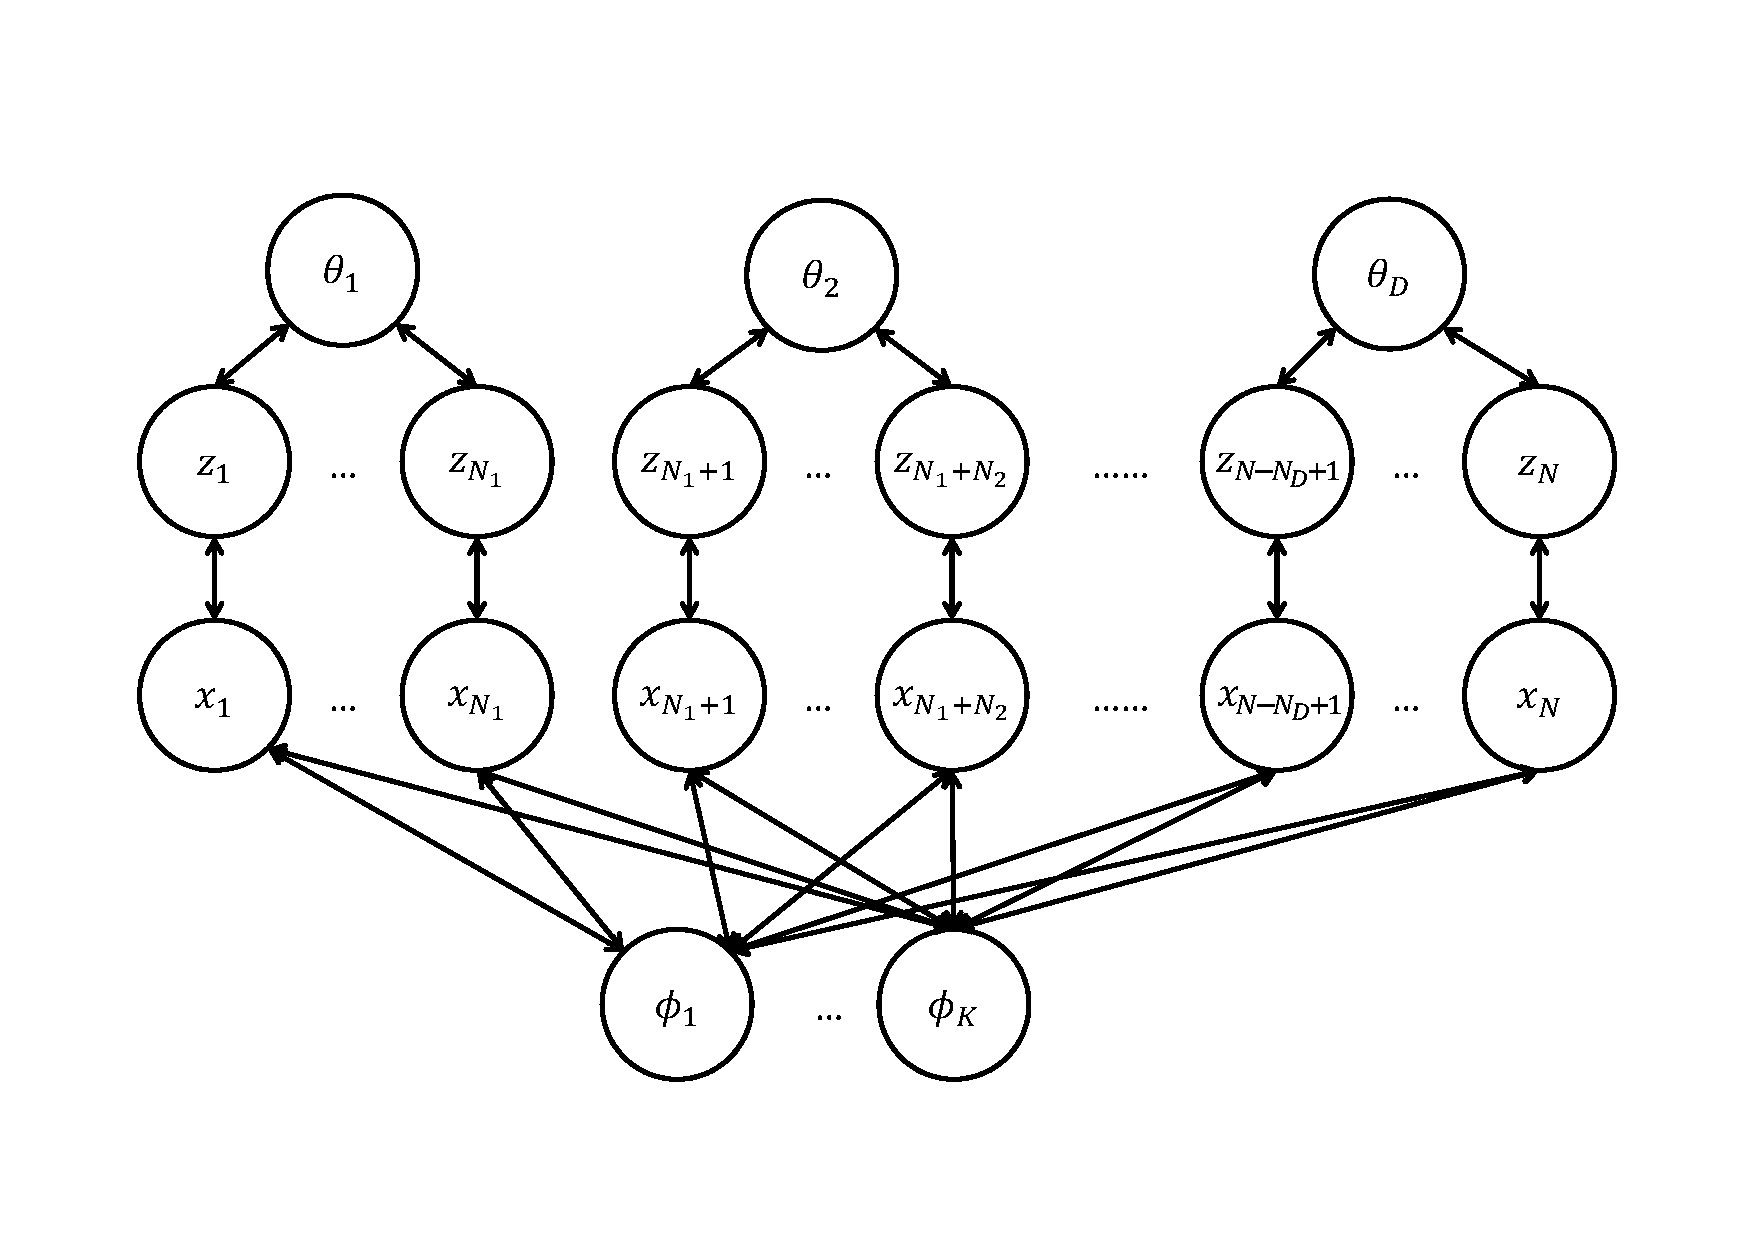
\includegraphics[width=0.45\textwidth]{figs/Graph1}
	\caption{Message Passing Graph of a Mixture Model}
	\label{fig:mixture_mpg}
\end{figure}

The four partition
strategies that we will examine
are all the ones provided by GraphX,
which are
(1) EdgePartition1D (1D),
(2) EdgePartition2D  (2D),
(3) RandomVertexCut (RVC), and
(4) CanonicalRandomVertexCut (CRVC).


%\figref{fig:mixture_mpg} shows a more typical message passing graph of a
%mixture model instead of the toy two-coin model that we have used so far.


EdgePartition1D essentially is a random partitioning strategy, except that it
co-locates all the edges with the same source vertex. Suppose all the edges from
$\phi_k$ are assigned to partition $k$. Since there's an edge from $\phi_k$ to
each one of the $N$ vertices $x$, partition $k$ will have the replications
of all $x_1, x_2, \ldots, x_N$. In the best case,
edges from different $\phi_k$ are assigned to different
partitions. Then the largest edge partition still have at least $N$ vertices.
When $N$ is very large, the largest edge partition is also very large, which
will easily cause the size of an edge partition to exceed the RDD block size limit. However,
the best case turns out to be the worst case
when it comes to the number of vertex replications
because it actually replicates the size $N$ data $K$ times, which is
extremely space inefficient. The over-replication also incurs large amount of
shuffling when we perform outer joins because each updated vertex has to
be shipped to every edge partition, prolonging the running time.

%We give a more formal analysis of the number of vertices in the largest edge
%partition and the expected number of replications of $x_i$ under
%EdgePartition1D.
As discussed above, there is at least one edge partition that
has replications of all the $x_i$'s.
Observe that the graph has an upper bound of
$3N + K$ vertices, so the number of vertices in the largest edge partition is
$O(N)$. Let $N_{x_i}$ be the number of replications of $x_i$
and $M$ be the number of partitions (which is usually a factor of the number of machines),
then the expected
number of replication of $x_i$ is
\begin{align*}
	E[N_{x_i}] &= M(1 - (1 - \frac{1}{M})^{K+1}) \\
		&= \left\{
			\begin{array}{ll}
				(K + 1) + o(1) & K = O(1) \\
				M + o(1) & K = O(M)
			\end{array}
		\right.%}
\end{align*}


%first introduction
%then analysis
\begin{figure}[h]
	\centering
	\includegraphics[scale=0.25]{figs/2dhash.eps}
	\caption{EdgePartition2D. Each grid is a partition.
	The possible partitions where $x_i$ is
	replicated is shaded}
	\label{fig:2dhash}
\end{figure}

EdgePartition2D evenly divides the adjacency matrix of the graph into $\sqrt{M}
\times \sqrt{M}$ partitions. The vertices are uniformly distributed along the
edges of the adjacency matrix by hashing into $\sqrt{M}$ buckets. The upper
bound of the number of replications of a vertex $x_i$ is $\sqrt{M}$ because all
the edges that point to it are distributed to at most $\sqrt{M}$ partitions
in shown as \figref{fig:2dhash}.  Meanwhile, there are $K+1$
edges pointing to $x_i$, so the number of replications of $x_i$ cannot exceed
$K+1$ as well. Therefore, the upper bound of replications of $x_i$ is actually
$\min(K+1, \sqrt{M})$. On the other hand, suppose each of the $\phi_k$ is
hashed to different bucket and $N$ $x$'s are evenly distributed into the
$\sqrt{M}$ buckets, then the number of largest partition is at least
$\frac{N}{\sqrt{M}}$, which is still huge when the average number of words per
partition is fixed. Following is the formal analysis of the EdgePartition2D.

Let $B$ be an arbitrary
partition in the dark column on \figref{fig:2dhash}.
Let $Y_{x_i, B}$ be the indicator variable for the event that $x_i$ is replicated in
Then the expectation of $Y_{x_i, B}$ is
\begin{align*}
	E[Y_{x_i, B}] &= 1 - (1 - \frac{1}{\sqrt{M}})^{K+1} \\
\end{align*}

The number of vertices $N_B$ in the largest partition $B$ is at least the expectation
of the number of vertices in a partition, which is also at least the
expectation of the number of $x_i$ in it:
\begin{align*}
	E[N_{B}] &= \sum_{v} E[Y_{v, B}] \\
		&\ge \frac{N}{\sqrt{M}} E[Y_{x_i, B}]	\\
		& = \left\{
				\begin{array}{ll}
					(K + 1)\eta	+ o(1) & K = O(1) \\
					\sqrt{M}\eta + o(1) & K = O(M)
				\end{array}
			\right.%}
\end{align*}

The expected number of replications of $x_i$ is
\begin{align*}
	E[N_{x_i}] &= \sqrt{M}E[Y_{x_i, B}] \\
		&= \left\{
			\begin{array}{ll}
				(K + 1) + o(1) & K = O(1) \\
				\sqrt{M} + o(1) & K = O(M)
			\end{array}
		\right.%}
\end{align*}


%
RandomVertexCut (RVC) uniformly assigns each edge to one of the $M$
partitions. The expected number of replications of $x_i$ tends to be $O(K)$
when $K$ is a constant and tends to be $O(N)$ when $K$ is proportional to the
number of partitions. The number of vertices in the largest partition is also
excessively large. It is $O(K\frac{N}{M})$ when K is a constant and $O(N)$
when $K$ is proportional to the number of partitions.  CanonicalRandomVertexCut
assigns two edges between the same pair of vertices with opposite directions
to the same partition. For VMP, it is the same as RandomVertexCut since only
the destination end of an edge is replicated. For example, if $x_i$ has $K +1$
incoming edges, then the probability that $x_i$ will be replicated in a
particular partition is independent from whether edges in opposite
direction are in the same partition or randomly distributed. Therefore
CRVC will have the same result as RVC.

InferSpark's partitioning strategy is actually tailor-made for message passing graphs.
The intuition is that the MPG has a special structure.
For example, in \figref{fig:mixture_mpg},
we see that the MPG essentially has $D$ ``independent'' trees rooted at $\theta_i$,
where the leaf nodes  are $x$'s and they form a complete bipartite graph with all $\phi$'s.
In this case, one good partitioning strategy is to form $D$ partitions,
with each tree going to one partition and the $\phi$'s getting replicated $D$ times.
Such a partition strategy incurs no replication on $\theta$, $z$, and $x$,
and incurs $D$ replications on $\theta$.





InferSpark's partitioning strategy is actually tailor-made for message passing graphs.
Its idea is as follows: Given an edge, we first determine
which two random variables (e.g. $x$ and $z$) are connected by the edge. It is
quite straightforward because we assign ID to the set of vertices of the same
random variable to a consecutive interval. We only need to look up which
interval it is in and what the interval corresponds to. Then we compare the
total number of vertices correponding to the two random variables and choose
the larger one. Let the Vertex ID range of the larger one to be $L$ to $H$. We
divide the range from $L$ to $H$ into $M$ subranges. The first subrange is $L$
to $L + \frac{H-L+1}{M}$; the second is $L + \frac{H-L+1}{M} + 1$ to $L +
2\frac{H-L+1}{M}$ and so on. If the vertex ID of the edge's chosen vertex falls
into the $m^{th}$ subrange, the edge is assigned to partition $m$.
In InferSpark, this partitioning strategy is generated
as a piece of code that embeds the above ID assignment scheme.


In the mixture case, at least one end of every edge is $z$ or $x$. Since
the number of $z$'s and $x$'s are the same,
each set of edges that link to the $z_i$ or $x_i$ with
the same $i$ are co-located. This guarantees that $z_i$
and $x_i$ only appears in one partition. All the $\phi_k$'s are replicated in each
of the $M$ partitions as before. The only problem is that many $\theta_j$ with
small $N_j$ could be replicated to the same location. In the worst case, the
number of $\theta$ in one single partition is exactly $\eta$. However, it is
not an issue in that case because the number of vertices in the largest
partition is still a constant $3\eta + K$. It is also independent from whether $K
= O(1)$ or $K = O(M)$.
Having that said, we now can also conclude the analysis of our partition strategy
and we give a summary in
\tabref{tab:max_v_per_edge_part_O1} and
\tabref{tab:max_v_per_edge_part_OM}.




\begin{table}[h]
	\centering
	\caption{Analysis of Different Partition Strategies When $K = O(1)$}
	\label{tab:max_v_per_edge_part_O1}
	\small
	\begin{tabular}{lll}
		\hline
		Partition Strategy & $E[N_{x_i}]$ & $E[N_B]$\\\hline\hline
		1D & $O(K)$ & $O(N)$ \\\hline
		2D & $O(K)$ & $O(K\frac{N}{M})$ \\\hline
		RVC & $O(K)$ & $O(K\frac{N}{M})$ \\\hline
		CRVC & $O(K)$ & $O(K\frac{N}{M})$ \\\hline
		{\bf InferSpark} & 1 & $3\frac{N}{M}+1$ \\\hline
	\end{tabular}
\end{table}

\begin{table}[h]
	\centering
	\caption{Analysis of Different Partition Strategies When $K = O(M)$}
	\label{tab:max_v_per_edge_part_OM}
	\small
	\begin{tabular}{lll}
		\hline
		Partition Strategy & $E[N_{x_i}]$ & $E[N_B]$\\\hline\hline
		1D & $O(M)$ & $O(N)$ \\\hline
		2D & $O(\sqrt{M})$ & $O(\sqrt{M}\frac{N}{M})$ \\\hline
		RVC & $O(M)$ & $O(N)$ \\\hline
		CRVC & $O(M)$ & $O(N)$ \\\hline
		{\bf InferSpark} & 1 & $3\frac{N}{M}+1$ \\\hline
	\end{tabular}
\end{table}

\subsection{Inferspark Runtime}
\label{sec:optimize_shuffle}

%Next, we present a way of optimizing shuffling in GraphX. The optimization
%eliminates the majority of shuffle in InferSpark. The optimization involves a
%complete re-write of GraphX, but it keeps all the API of GraphX so the porting
%of InferSpark from GraphX to the optimized version is effortless.
%

Data shuffle is an expensive operation in a distributed system because it
involves a lot of random disk I/Os and large amount of network traffic between each
pair of workers. In the case of Apache Spark, either slow random disk I/O or
low network bandwidth is a bottleneck of the shuffle performance. In most
cases, the random I/O is the main contributing factor to the poor shuffle
performance although shuffle file consolidation mitigates the problem
\cite{spark-shuffle}.

The way that GraphX implements data shuffle is to simply re-partition the
vertices or messages according to the partitioner of the RDD to be zip-joined
with uses. GraphX first flat maps each vertex partition $i$ to an array of
vertex blocks. The vertices in block $j$ are the vertices that need to be
replicated in edge partition $j$.  Block $j$ is also paired with the partition
ID $j$ so that it can be re-partitioned using the edge RDD's partitioner.
Finally, GraphX calls ``partitionBy'' on the resulting RDD to get an RDD of
replicated vertices that is zip-joinable with the edge RDD.

Under our partitioning strategy, there is one single edge partition to which
most of the vertices are replicated, for each of the vertex partitions. The
shuffle size will be greatly reduced if these vertices are not actually
shuffled to the edge partitions.
%
%\begin{figure}
%	\centering
%	\includegraphics[scale=0.5,clip]{figs/graph_partition.eps}
%	\caption{InferSpark runtime}
%	\label{fig:inferspark_graph_partition}
%\end{figure}

Therefore, we implement our InferSpark runtime
as a PGM-aware vertex-edge co-location implementation of the GraphX API.
That is, the vertex partition is merged with the edge partition
so that most of the vertices are replicated into a single partition.
% (see
%\figref{fig:inferspark_graph_partition}).
%The replicated vertices in such a
%partition reduces to those were not in the vertex partition before the merge.
As a consequence,
we only need to shuffle those vertices that were not in the
corresponding vertex partition.
In the case of InferSpark, most vertices are referenced from only
one edge partition. Thus the optimization eliminates almost all the shuffle
during vertex replication.

%The change in the implementation does not necessarily break the GraphX API
%since we can still provide a Vertex RDD view and an Edge RDD view via
%projection. Hence, porting InferSpark to the optimized GraphX is effortless.


%
%
%Both the original GraphX and the optimized version persist some intermediate
%RDDs behind the scene for performance consideration, making it hard for the
%generated inference code to properly unpersist all the unnecessary cached
%RDDs. For example, the underlying RDD of GraphX prior to vertex replication is
%hidden when the vertex replication occurs. It will be persisted if the graph
%is persisted prior to vertex replication, wasting the precious memory of
%executors.
%
%We modified GraphX to keep track of the intermediate RDDs so that they are
%un-persisted whenever an action is invoked on the final RDD. With this feature,
%we can avoid persisted RDDs being accumulated in the cache.


